\section {Case Study: Transformer}

Hyper parameters are \textbf{literal constants}:
\begin{enumerate}
  \item $d = 512$: embedding dimension = hidden dimension
  \item $n_{\text{head}} = 8$: number of heads
  \item $d_{ff1} = 2048$
  \item $d_{ff2} = d = 512$
\end{enumerate}

Symbolic constants:
\begin{enumerate}
  \item $\text{batch\_size}$
  \item $L$: sequence length
\end{enumerate}

Notations:

\begin{itemize}
  \item $\otimes$: matrix multiplication
  \item $\textbf{Var}_{n}^{\text{tensor shape}}$: learnable parameter.
  \begin{itemize}
    \item $n$ is the index of learnable parameter.
    \item $\text{tensor\_shape}$ is the shape of learnable parameter.
    \item If $\text{tensor\_shape}$ is omitted and $\text{Var}$ is not in bold, such a learnable parameter is a scalar.
  \end{itemize}
  \item $\textbf{Y}_{n}^{\text{tensor shape}}$: produced intermediate result which is immutable in forward computation.
  \begin{itemize}
    \item $n$ index of the variable.
    \item $\text{tensor\_shape}$: shape of the variable.
    \item If $\text{tensor\_shape}$ is omitted and $Y$ is not in bold, such a variable is a scalar.
  \end{itemize}

\end{itemize}

\subsection{Basic Building Blocks}

\subsubsection {Positional encoding}

Can be fused into one element-wise kernel.

$$\mathbf{Y}_0^{d\times L}=\text{slice}(\mathbf{Token}^{L \times1}, \mathbf{Var}_{0}^{d\times \text{vocab\_size}}, \text{dim}=1) .* \sqrt{d} .+ \mathbf{PosEnc}^{d\times L}$$

\subsubsection{Multi-head attention}

Below is the equation for multi-head self-attention which suppress various details of computation process.

\begin{equation}
  \text{Attention}(\mathbf{Q},\mathbf{K},\mathbf{V}) =
  \text{softmax}(\frac{\mathbf{Q}\mathbf{K}^T}{\sqrt{d}})\mathbf{V} \label{eq1}
\end{equation}

\begin{enumerate}
  \item $\mathbf{Y}_1^{d \times L}=\mathbf{Var}_{1}^{d \times d} \otimes \mathbf{Y}_0^{d \times L}$

  \item $\mathbf{Y}_2^{d \times L}=\mathbf{Var}_{2}^{d \times d} \otimes \mathbf{Y}_0^{d \times L}$

  \item $\mathbf{Y}_3^{d \times L}=\mathbf{Var}_{3}^{d \times d} \otimes \mathbf{Y}_0^{d \times L}$

  \item $\mathbf{Y}_4^{n_1 \times n_2 \times L} = \textbf{reshape}(\mathbf{Y}_1^{d \times L}, (n_1, n_2, L))$
  \begin{itemize}
    \item $n_1 = n_{\text{head}}$, $n_2 = d // n_{\text{head}}$;
    \item the $\mathbf{Q}$ part in equation \eqref{eq1};
  \end{itemize}

  \item $\mathbf{Y}_5^{n_1 \times n_2 \times L} = \textbf{reshape}(\mathbf{Y}_2^{d \times L}, (n_1, n_2, L))$
  \begin{itemize}
    \item $n_1 = n_{\text{head}}$, $n_2 = d // n_{\text{head}}$;
    \item the $\mathbf{K}$ part in equation \eqref{eq1};
  \end{itemize}

  \item \begin{equation*}
    \begin{aligned}
    \mathbf{Y}_8^{n_1 \times L \times L} = \textbf{parallel\_foreach}(&\mathbf{Y}_{6i}^{n_2 \times L}, \mathbf{Y}_{7i}^{n_2 \times L} \quad \textbf{in} \quad \mathbf{Y}_4[i,:,:], \mathbf{Y}_5[i,:,:]) \text{,} \quad i \in [0,1,...,n_1 - 1] \\
    & \mathbf{Y}_{8i}^{L \times L} = (\mathbf{Y}_{6i}^{n_2 \times L})^{T} \otimes \mathbf{Y}_{7i}^{n_2 \times L}
    \end{aligned}
  \end{equation*}

  \item $\mathbf{Y}_9^{n_1 \times L \times L} = \mathbf{Y}_8^{n_1 \times L \times L} .* \sqrt{d}$
  \item $\mathbf{Y}_{10}^{n_1 \times L \times L} = \textbf{apply\_along\_axis}(\text{softmax}, 1, \mathbf{Y}_9^{n_1 \times L \times L})$

  \item $\mathbf{Y}_{11}^{n_1 \times n_2 \times L} = \textbf{reshape}(\mathbf{Y}_4^{d \times L}, (n_1, n_2, L))$
  \begin{itemize}
    \item $n_1 = n_{\text{head}}$, $n_2 = d // n_{\text{head}}$;
    \item the $\mathbf{V}$ part in equation \eqref{eq1};
  \end{itemize}

  \item \begin{equation*}
    \begin{aligned}
    \mathbf{Y}_{12}^{n_1 \times n_2 \times L} = \textbf{parallel\_foreach} ( &\mathbf{Y}_{13i}^{n_2 \times L}, \mathbf{Y}_{14i}^{n_2 \times L} \quad \textbf{in} \quad \mathbf{Y}_{11}[i,:,:], \mathbf{Y}_{10}[i,:,:]) \text{,} \quad i \in [0,1,...,n_1 - 1] \\
    & \mathbf{Y}_{12i}^{n_2 \times L} = \mathbf{Y}_{13i}^{n_2 \times L} \otimes \mathbf{Y}_{14i}^{L \times L}
    \end{aligned}
  \end{equation*}

  \item $\mathbf{Y}_{15}^{d \times L} = \textbf{reshape}(\mathbf{Y}_{12}^{d \times L}, (n_1 * n_2, L))$

\end{enumerate}

\begin{info}

$\mathbf{Y}^{N} = \text{softmax}(\mathbf{X}^N)$
\begin{enumerate}
  \item $Y_0 = \textbf{reduce}(\text{max}, \mathbf{X}^N)$
  \item $\mathbf{Y}_1^{N} = \textbf{broadcast}(-, \mathbf{X}^N, Y_0)$
  \item $\mathbf{Y}_2^{N} = \textbf{parallel\_foreach}(\text{exp}, \mathbf{Y}_1^N)$
  \item $Y_3 = \textbf{reduce}(\text{+}, \mathbf{Y}_2)$
  \item $\mathbf{Y}_4^{N} = \textbf{broadcast}(/, \mathbf{Y}_2^{N}, Y_3)$
\end{enumerate}
\end{info}

\subsubsection{Add and norm}

\begin{enumerate}
  \item $\mathbf{Y}_{16}^{d \times L} = \textbf{parallel\_foreach}(+, \mathbf{Y}_{15}^{d \times L}, \textbf{PosEnc}^{d \times L})$
  \item $\mathbf{Y}_{17}^{d \times L} = \textbf{apply\_along\_axis}(\text{norm},0,\mathbf{Y}_{16}^{d \times L})$
  \item $\mathbf{Y}_{18}^{d \times L} = \textbf{broadcast}(*, \mathbf{Y}_{17}^{d \times L}, \text{Var}_4)$
  \item $\mathbf{Y}_{19}^{d \times L} = \textbf{broadcast}(+, \mathbf{Y}_{18}^{d \times L}, \text{Var}_5)$
\end{enumerate}

\begin{info}

$\mathbf{Y}^{N} = \text{norm}(\mathbf{X}^N)$.
\begin{enumerate}
  \item $Y_0 = \textbf{reduce}(+, \mathbf{X}^N) / N$
  \begin{itemize}
    \item mean
  \end{itemize}
  \item $\textbf{Y}_1^{N} = \textbf{broadcast}(-, \mathbf{X}^{N},\textbf{Y}_0)$
  \item $\textbf{Y}_2^{N} = \textbf{parallel\_foreach}(\textbf{pow}, \mathbf{Y}_1^{N}, 2)$
  \item $Y_3 = \textbf{reduce}(+, \mathbf{Y}_2^N)$
  \item $Y_4 = \text{sqrt}(Y_3 / N)$
  \begin{itemize}
    \item variance
  \end{itemize}
  \item $Y_5 = \textbf{parallel\_foreach}(x \rightarrow (x-Y_0)/(Y_5 + \epsilon),\mathbf{X}^N)$
\begin{itemize}
  \item $\epsilon = 1e^{-6}$ is a constant.
\end{itemize}
\end{enumerate}
\end{info}

\subsubsection{Pointwise feed forward}

$$\text{FFN}(\mathbf{X}) = \text{max}(0, \mathbf{X}\mathbf{W}_1 + \mathbf{b}_1)\mathbf{W}_2 + \mathbf{b}_2$$

\begin{enumerate}
  \item $\mathbf{Y}_{20}^{L \times d_{ff1}} = (\mathbf{Y}_{19}^{d \times L})^T \otimes \mathbf{Var}_6^{d \times d_{ff1}}$
  \item $\mathbf{Y}_{21}^{L \times d_{ff1}} = \textbf{broadcast}(+, \mathbf{Y}_{20}^{L \times d_{ff1}}, \mathbf{Var}_{7}^{d_{ff1}})$
  \item $\mathbf{Y}_{22}^{L \times d_{ff1}} = \textbf{parallel\_foreach}(\text{relu}, \mathbf{Y}_{21}^{L \times d_{ff1}})$
  \begin{itemize}
    \item relu is a scalar function:\begin{equation*}
    \begin{aligned}
      \text{relu}(x) = \left\{
      \begin{aligned}
        &x \quad x > 0 \\
        &0 \quad \text{otherwise}
      \end{aligned}
      \right. \\
    \end{aligned}
  \end{equation*}
  \end{itemize}

  \item $\mathbf{Y}_{23}^{L \times d_{ff1}} = \textbf{parallel\_foreach}(\text{dropout}, \mathbf{Y}_{22}^{L \times d_{ff1}},\text{drop\_rate=0.5})$
  \begin{itemize}
    \item dropout is a scalar function:\begin{equation*}
    \begin{aligned}
      \text{dropout}(x, \text{drop\_rate}) = \left\{
      \begin{aligned}
        &x \quad \text{random()} \le \text{drop\_rate} \\
        &0 \quad \text{otherwise}
      \end{aligned}
      \right. \\
    \end{aligned}
  \end{equation*}

  \end{itemize}
  \item $\mathbf{Y}_{24}^{L \times d} = \mathbf{Y}_{23}^{L \times d_{dff1}} \otimes \textbf{Var}_{8}^{d_{ff1} \times d}$
  \item $\mathbf{Y}_{25}^{L \times d} = \textbf{broadcast}(+, \mathbf{Y}_{24}^{L \times d}, \textbf{Var}_{9}^{d})$
\end{enumerate}

\subsection{Optimizations}

\begin{figure}[htbp]
\centering
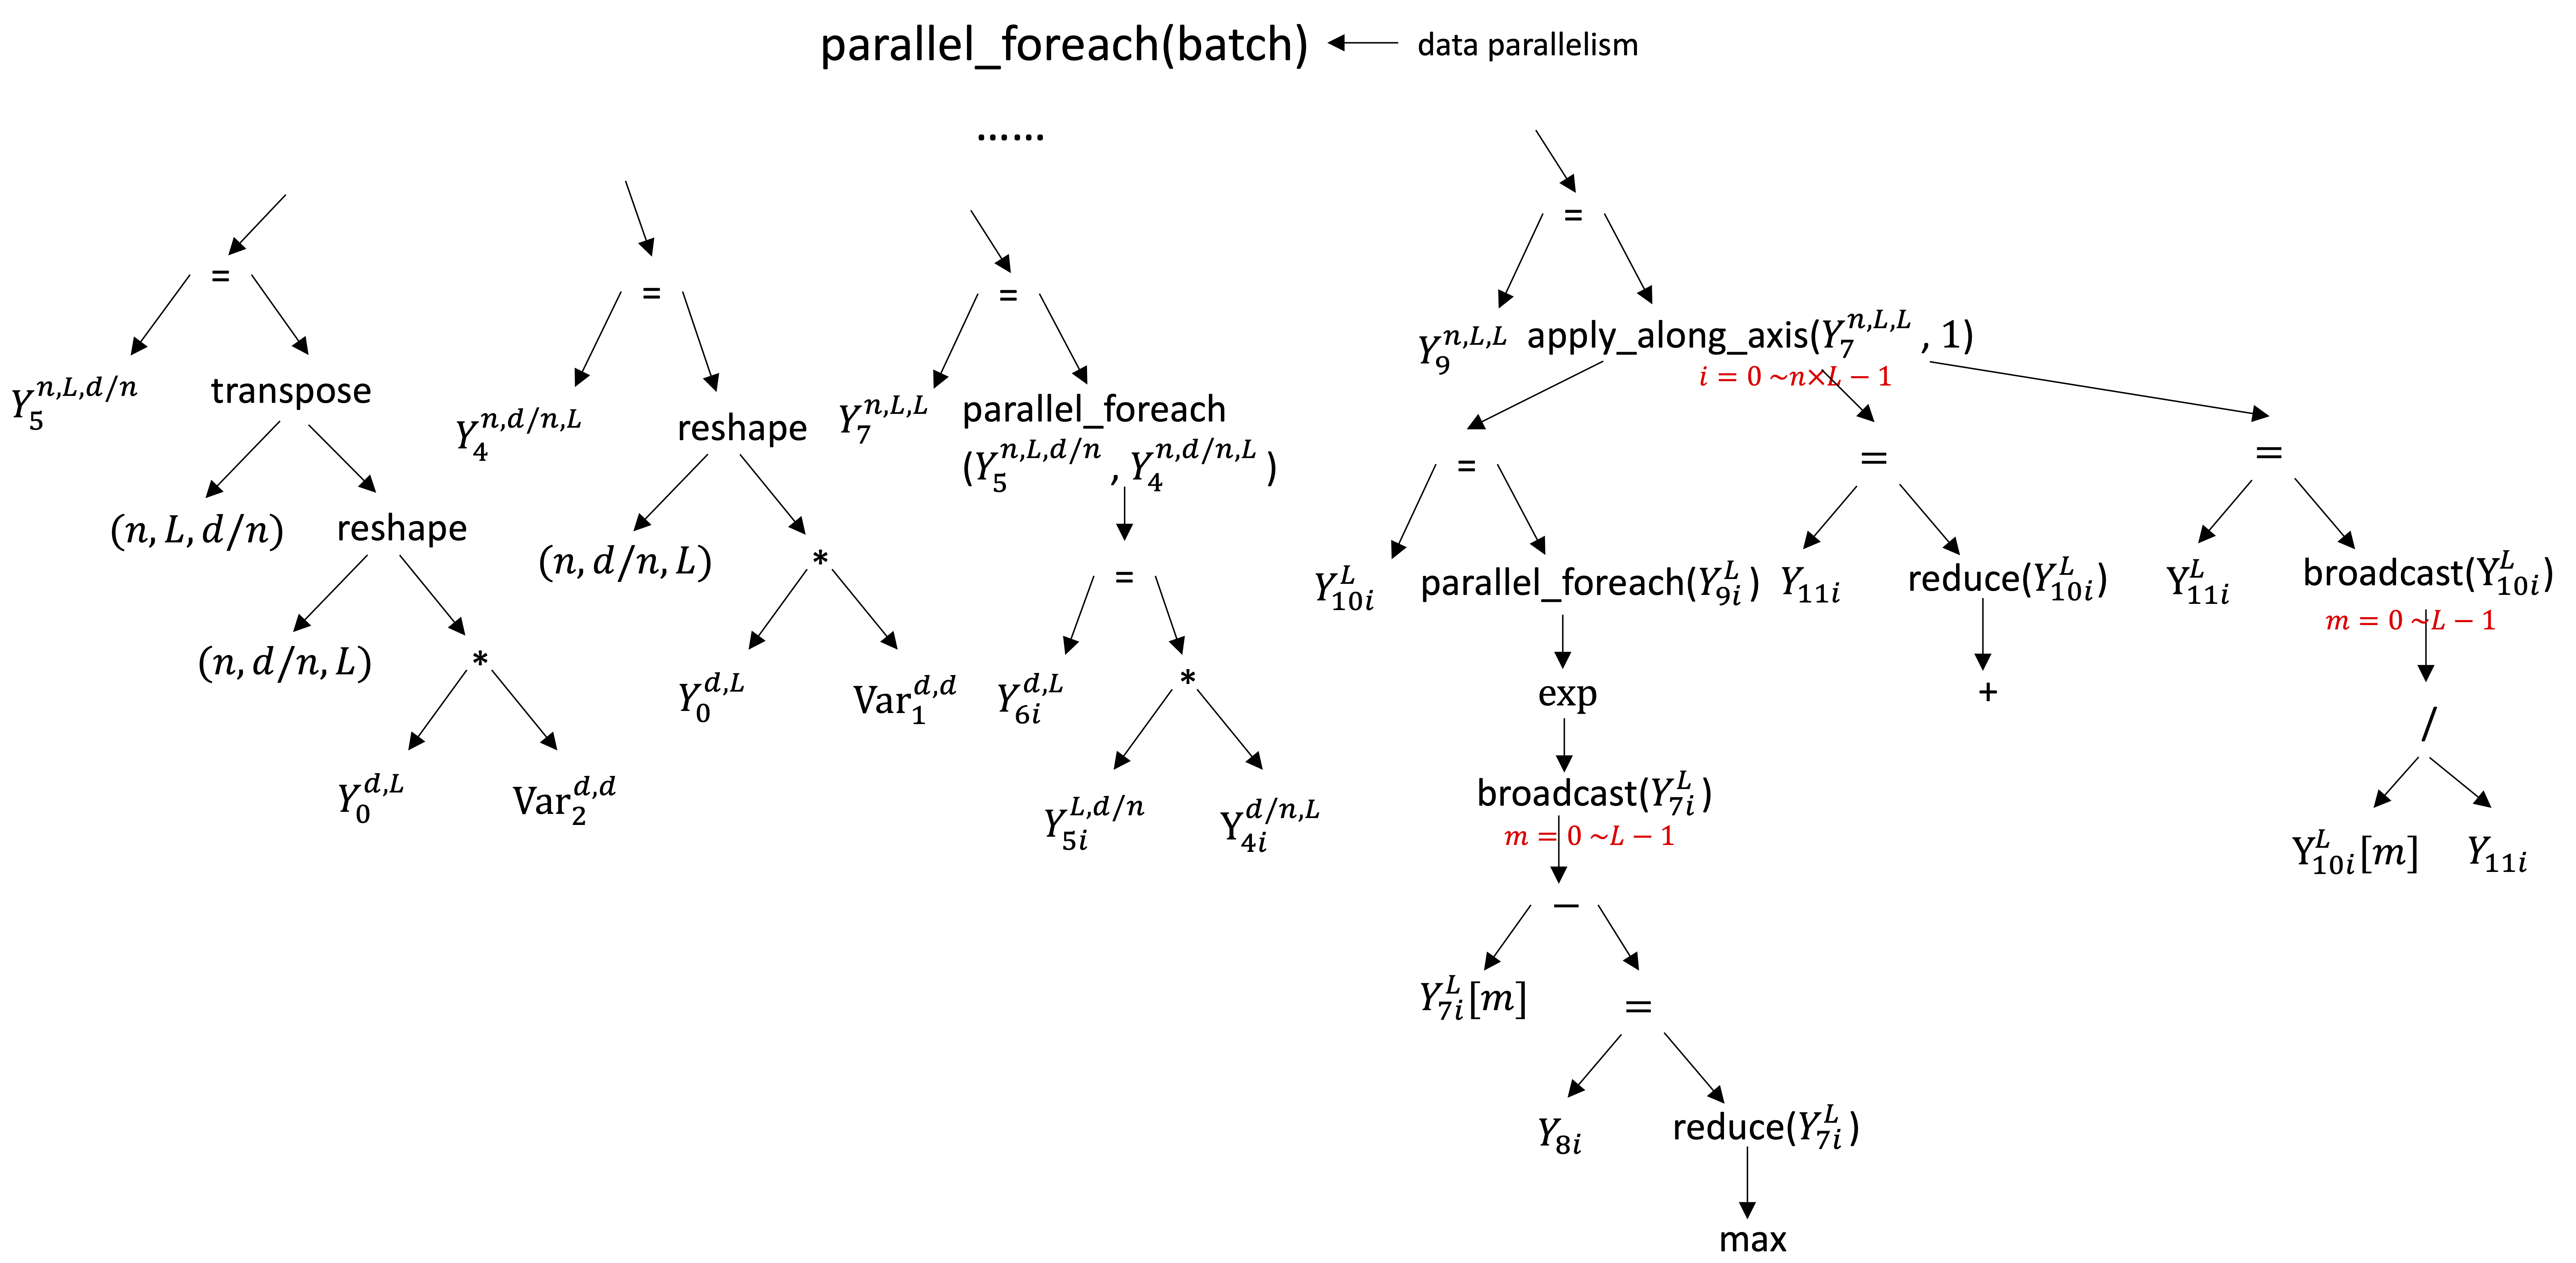
\includegraphics[width=1.\textwidth]{images/transformer.png}
\caption{AST for $\text{softmax}(K^TQ)$}
\label{Fig.}
\end{figure}

\subsubsection {Loop fusion}

\subsubsection {Loop distribution}

\subsubsection {Data movement removal (layout optimization)}

\subsubsection {CSE}

\subsubsection {Auto-batching of variable-length sequences}
